\section[Introdução]{Introdução}

O projeto Soul Amada \cite{projeto-soul-amada} foi concebido com o propósito de promover a saúde mental de mulheres no Brasil, incentivando práticas de meditação e fortalecendo a conexão espiritual. A principal stakeholder e responsável pelo projeto foi a Dayanne Silveira Antunes.

A saúde mental representa um desafio significativo em nível global, com efeitos
particulares sobre as mulheres e sobre pessoas que não conseguem acesso adequado
a prevenção, acolhimento e tratamento. Dificuldades como ansiedade e depressão
podem ser agravadas quando a necessidade de ajuda profissional não é reconhecida
ou quando esse atendimento não está disponível.

Diante desse cenário, o projeto Soul Amada foi concebido para oferecer apoio emocional e espiritual a mulheres no Brasil. Reconhecendo a influência de crenças, hábitos e comportamentos na saúde mental, a iniciativa busca ser uma fonte de orientação e incentivo para mulheres que enfrentam ansiedade, depressão e outros desafios emocionais.

O principal objetivo então do Soul Amada é o desenvolvimento de um aplicativo mobile que promova o crescimento pessoal e espiritual das usuárias. Por meio de conteúdos diários, o aplicativo oferecerá informações relevantes, incentivo à prática de hábitos saudáveis e suporte para lidar com desafios emocionais. Com foco na transformação de vidas, a plataforma também servirá como um guia para ajudar as usuárias a compreenderem a importância de buscar ajuda profissional quando necessário, fortalecendo seu bem-estar geral e promovendo uma conexão mais profunda com sua espiritualidade.

O time do projeto, apresentado na Figura~\ref{fig:projeto-time2}, contou com
a orientação e o suporte da Prof.ª Dra. Cristina Moreira Nunes. As datas de
início e fim do projeto foram de 15/08/2023 a 21/11/2023.


\begin{figure}[H]
  \centering
  \small
  \caption{Time do projeto Soul Amada}
  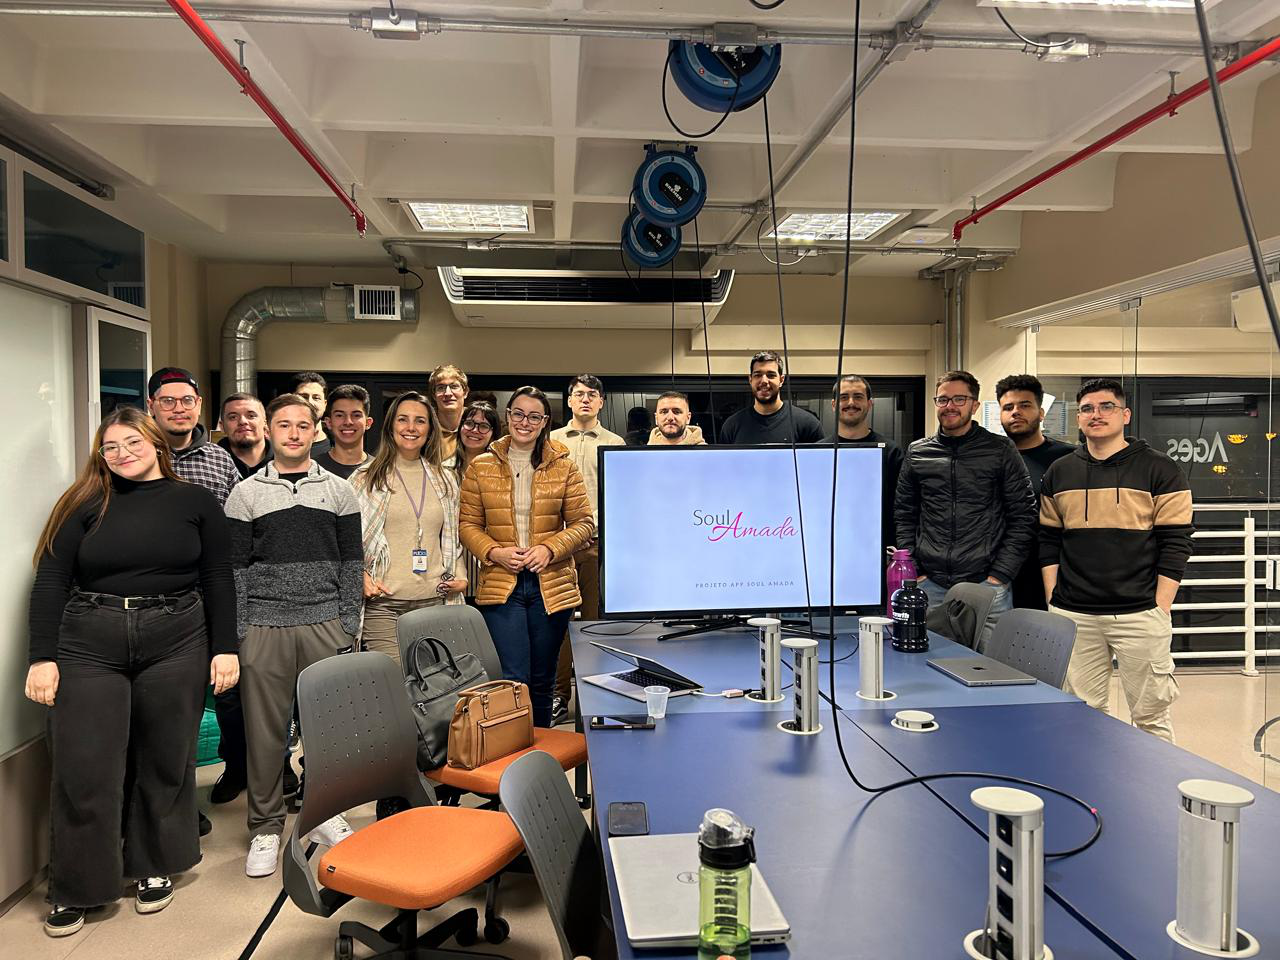
\includegraphics[width=1\linewidth]{conteudo//3 - ages II//conteudo//figures/foto-time.png}
  Fonte: Autor
  \label{fig:projeto-time2}
\end{figure}